\documentclass[aspectratio=169,11pt]{beamer}
\usepackage[T1]{fontenc}
\usepackage{lmodern}
\usepackage{listings}
\usepackage{booktabs}
\usepackage{tikz}
\usetikzlibrary{arrows.meta,positioning}
\definecolor{Ink}{HTML}{172B4D}
\definecolor{Teal}{HTML}{007F86}
\definecolor{Rust}{HTML}{B64B2B}
\definecolor{Mist}{HTML}{F1F5F8}
\setbeamercolor{normal text}{fg=Ink,bg=white}
\setbeamercolor{structure}{fg=Teal}
\setbeamercolor{frametitle}{fg=Ink}
\setbeamercolor{title}{fg=Ink}
\setbeamercolor{block title}{fg=white,bg=Teal}
\setbeamercolor{block body}{bg=Mist}
\setbeamercolor{alerted text}{fg=Rust}
\setbeamertemplate{navigation symbols}{}
\setbeamertemplate{itemize items}[circle]
\setbeamertemplate{footline}{\hspace{6mm}\scriptsize\insertsectionhead\hfill\insertframenumber\,/\,\inserttotalframenumber\hspace{6mm}\vspace{4mm}}
\setbeamersize{text margin left=9mm,text margin right=9mm}
\setbeamerfont{frametitle}{size=\Large,series=\bfseries}
\setbeamerfont{title}{size=\Huge,series=\bfseries}
\lstdefinelanguage{Verus}{keywords={fn,let,mut,if,else,while,return,use,pub,as,requires,ensures,invariant,decreases,spec,proof,assert,true,false},morecomment=[l]{//},morestring=[b]"}
\lstset{language=Verus,basicstyle=\ttfamily\small,keywordstyle=\color{Teal}\bfseries,commentstyle=\color{gray},stringstyle=\color{Rust},backgroundcolor=\color{Mist},frame=none,xleftmargin=2mm,xrightmargin=2mm,aboveskip=2mm,belowskip=2mm,showstringspaces=false,columns=fullflexible,keepspaces=true}
\newcommand{\source}[2]{\vfill{\tiny\color{gray}Source: \href{#1}{#2}}}
\title{Code Verification in Rust with Verus}
\subtitle{Programs as mathematical objects; correctness as a theorem}
\author{}
\date{}
\begin{document}
\begin{frame}[plain]
\vspace{9mm}\titlepage
\end{frame}

\section{Introduction}
\begin{frame}{When an algorithm becomes a program}
\Large A proof about an algorithm is a starting point.\par
\medskip What theorem does its implementation satisfy?
\vspace{5mm}\normalsize
\begin{itemize}
\item Specify the domain, hypotheses, and desired conclusion.
\item Model execution as a relation between states.
\item Prove that every permitted execution preserves the claim.
\end{itemize}
\begin{block}{Today's example}A bounded successor: increment an integer until it reaches a limit.\end{block}
\note{Audience: a graduate mathematics department. Assume comfort with proofs, quantifiers, and induction; assume no Rust knowledge or specialist training in logic. Aim for 30--35 minutes plus questions. Motivate with the gap between a mathematical algorithm and its finite-machine implementation.}
\end{frame}

\begin{frame}{The route}
\tableofcontents
\note{Timing: introduction 4 minutes; verification 7; Z3 6; Verus 10; LLM guardrails 6. Emphasize the logical translation and induction argument. The same bounded-successor example connects the sections.}
\end{frame}

\begin{frame}{A bounded successor: the intended mathematics}
For a fixed $L\in\mathbb{N}$, define
\[
 f_L:\{0,\ldots,L\}\longrightarrow\{0,\ldots,L\},\qquad
 f_L(x)=\min(x+1,L).
\]
\begin{block}{A tempting implementation}
\[g_L(x)=\begin{cases}x+1 & x\le L,\\x & x>L.\end{cases}\]
\end{block}
At $x=L$, we obtain $g_L(L)=L+1$: the claimed codomain is violated.
\medskip\par
We want a proof of $\forall x\in\{0,\ldots,L\},\ g_L(x)=f_L(x)$\textemdash or a counterexample.
\note{Start with familiar mathematics rather than unfamiliar syntax. The error is deliberately elementary: the interesting question is how to turn its detection into a mechanical procedure. A few successful evaluations do not establish the universally quantified claim.}
\end{frame}

\section{What is code verification}
\begin{frame}{Turn intent into a contract}
\begin{columns}[T]
\column{.48\textwidth}
\begin{block}{Precondition: caller's obligation}
$x \le \mathit{limit}$
\end{block}
\begin{block}{Postcondition: callee's promise}
$r \le \mathit{limit}$\par\medskip
$r=\begin{cases}x+1 & x<\mathit{limit}\\x & x=\mathit{limit}\end{cases}$
\end{block}
\column{.48\textwidth}
\large The contract says both:
\normalsize\begin{itemize}
\item what inputs are allowed;
\item exactly how the result relates to the input.
\end{itemize}
\medskip A bound alone is too weak: returning zero would satisfy it.
\end{columns}
\note{These equations use mathematical integers. Later, Verus must additionally establish that executable u32 arithmetic is safe. Preconditions restrict the promise; they do not validate external input at runtime.}
\end{frame}

\begin{frame}{Hoare triples are statements about executions}
Let $s$ and $s'$ denote program states, and let $C(s,s')$ mean that\par
program $C$ can terminate in $s'$ when started in $s$.
\[
 \{P\}\ C\ \{Q\}
 \quad\Longleftrightarrow\quad
 \forall s,s',\ P(s)\land C(s,s')\Longrightarrow Q(s').
\]
\begin{itemize}
\item $P$: a predicate on the initial state (the precondition).
\item $Q$: a predicate on the final state (the postcondition).
\item Initial values can be retained in the state to express input--output relations.
\end{itemize}
\begin{block}{Partial versus total correctness}This statement constrains terminating executions.\par Total correctness additionally requires termination on permitted inputs.\end{block}
\note{This is a semantic reading of the Hoare triple. C is a relation, not necessarily a total function. A nonterminating computation has no final state, so the implication alone cannot rule it out. Safety conditions such as overflow must also be represented or checked separately.}
\end{frame}

\begin{frame}{From assignments to proof obligations}
To establish $Q$ after an assignment $x:=e$, establish $Q[e/x]$ before it:
\[
 \{Q[e/x]\}\ x:=e\ \{Q\}.
\]
For example, with $Q(x)\equiv x\le L$ and $e=x+1$,
\[
 Q[e/x]\equiv x+1\le L.
\]
\begin{block}{A branch supplies a hypothesis}
Over $\mathbb{Z}$, the guard $x<L$ implies $x+1\le L$.\par
The guard $x\le L$ does not.
\end{block}
\note{Here Q[e/x] denotes capture-avoiding substitution. For this pure assignment over mathematical integers, it is the weakest precondition. Machine arithmetic adds definedness and range obligations. The implication uses discreteness: over the reals x < L would not be sufficient for x + 1 <= L.}
\end{frame}

\begin{frame}{The statement of the theorem matters}
\begin{itemize}
\item \textbf{Too weak:} $0\le r\le L$ is also satisfied by $r=0$.
\item \textbf{Vacuous:} an inconsistent $P$ makes $P\Rightarrow Q$ valid for any $Q$.
\item \textbf{Wrong structure:} arithmetic in $\mathbb{Z}$ differs from arithmetic modulo $2^{32}$.
\end{itemize}
\begin{block}{Two separate questions}
Does the implementation satisfy the formal specification?\par
Does the formal specification express the intended mathematics?
\end{block}
\note{Compare this with proving a theorem under accidentally contradictory hypotheses, or proving a statement in the wrong category of objects. Formal verification checks the formal claim; choosing the right claim remains mathematical work.}
\end{frame}

\section{Z3}
\begin{frame}{Z3: satisfiability relative to a theory}
\begin{block}{SMT: satisfiability modulo theories}
Given a formula $\varphi$ and background theory $T$, is there a model\par
$\mathcal{M}\models T$ and an assignment $\alpha$ such that $\mathcal{M},\alpha\models\varphi$?
\end{block}
\begin{itemize}
\item Boolean combinations of constraints in supported theories.
\item Examples: integer arithmetic, fixed-width bit-vectors, arrays.
\item The theory determines the meaning of symbols such as $+$ and $\le$.
\end{itemize}
\medskip For our example: linear constraints over the integers.
\source{https://microsoft.github.io/z3guide/}{Microsoft's Z3 Guide}
\note{No model-theory background is required: read a model as a structure in which all the constraints hold. For the integer example the domain and operations have their standard arithmetic interpretation; the unknowns are values assigned to x and L.}
\end{frame}

\begin{frame}{Prove a property by searching for its violation}
\[\neg\exists s,s':\ P(s)\land C(s,s')\land\neg Q(s').\]
Ask whether the existential counterexample formula is satisfiable.
\begin{center}
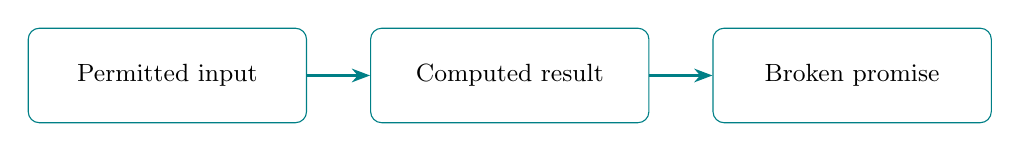
\begin{tikzpicture}[node distance=8mm, every node/.style={font=\small},box/.style={draw=Teal,rounded corners,align=center,minimum height=12mm,text width=33mm}]
\node[box] (p) {Permitted input};
\node[box,right=of p] (c) {Computed result};
\node[box,right=of c] (q) {Broken promise};
\draw[-{Stealth},thick,Teal] (p)--(c);
\draw[-{Stealth},thick,Teal] (c)--(q);
\end{tikzpicture}
\end{center}
\begin{itemize}
\item \texttt{sat}: a violation exists in this encoding.
\item \texttt{unsat}: no such violation exists in this encoding.
\item \texttt{unknown}: the solver could not decide; no proof obtained.
\end{itemize}
\source{https://microsoft.github.io/z3guide/docs/logic/basiccommands/}{Z3 Guide: Basic Commands}
\note{A timeout also leaves the obligation unproved. With abstractions, a satisfying model may require interpretation before calling it a real program counterexample. Our small exact arithmetic example has a direct interpretation.}
\end{frame}

\begin{frame}[fragile]{Ask Z3 for the boundary bug}
\begin{lstlisting}[language={},basicstyle=\ttfamily\small]
(set-logic QF_LIA)
(declare-const x Int)
(declare-const limit Int)
(assert (and (<= 0 x) (<= x limit)
             (<= limit 4294967295)))
(define-fun r () Int (ite (<= x limit) (+ x 1) x))
(assert (> r limit)) ; violate the bound
(check-sat)
(get-model)
\end{lstlisting}
\texttt{sat}: for example, $x=0$, $\mathit{limit}=0$ gives $r=1$.
\note{Read prefix notation aloud: (<= x limit) means x <= limit; ite means if-then-else. \texttt{QF\_LIA} selects quantifier-free linear integer arithmetic. Free constants are assigned values in a satisfying model, so the query searches existentially. This is examples/counter-bug.smt2; the exact model may differ.}
\end{frame}

\begin{frame}[fragile]{Change the branch condition; check again}
\begin{lstlisting}[language={}]
(define-fun r () Int (ite (< x limit) (+ x 1) x))
(assert (> r limit))
(check-sat)
; unsat
\end{lstlisting}
\begin{itemize}
\item In the increment branch: $x<\mathit{limit}$ implies $x+1\le\mathit{limit}$.
\item Otherwise: $x\le\mathit{limit}$ implies $x=\mathit{limit}$.
\item The input bound also gives $r\le 2^{32}-1$.
\end{itemize}
\medskip This query proves the bound. A complete contract also fixes the exact result.
\note{The full standalone query is in examples/counter-fixed.smt2. It uses the same input assertions as the previous slide. Verus automates generation of obligations from the source instead of requiring us to manually maintain this encoding.}
\end{frame}

\begin{frame}{Automation depends on the logical fragment}
\begin{itemize}
\item Our query uses quantifier-free linear integer arithmetic.
\item General quantified formulas require more than arithmetic simplification.
\item Nonlinear arithmetic can also make proof search difficult.
\item Auxiliary lemmas expose intermediate facts the search needs.
\end{itemize}
\begin{block}{Failure to prove is not a disproof}
A countermodel, an inconclusive answer, and a timeout are different outcomes.
\end{block}
\source{https://microsoft.github.io/z3guide/docs/logic/Quantifiers/}{Z3 Guide: Quantifiers}
\note{A specialist may ask about decidability. Distinguish a decidable fragment from the whole verification language and from practical resource bounds. Do not suggest that SMT is a complete decision procedure for arbitrary mathematical statements. Quantifier instantiation is generally heuristic.}
\end{frame}

\section{Verus}

\begin{frame}[fragile]{Enough Rust to read the example}
\begin{lstlisting}
fn advance(x: u32, limit: u32) -> u32 {
    if x < limit { x + 1 } else { x }
}
\end{lstlisting}
\begin{itemize}
\item \texttt{fn}: define a function; \texttt{-> u32}: its output type.
\item \texttt{u32}: an integer in $\{0,\ldots,2^{32}-1\}$.
\item \texttt{if ... else ...}: choose an expression; the final expression is returned.
\end{itemize}
\begin{block}{Finite arithmetic introduces an obligation}
To execute \texttt{x + 1} without overflow, prove $x<2^{32}-1$.
\end{block}
\note{Rust is a systems programming language with static checks on types and memory use. We need no ownership or lifetime syntax in this talk. Ordinary u32 addition must not be treated as mathematical addition beyond its range: overflow behavior depends on settings, while explicit wrapping arithmetic is a different operation. Verus checks absence of overflow for the addition shown.}
\end{frame}

\begin{frame}{Verus connects Rust code to proof obligations}
\begin{center}
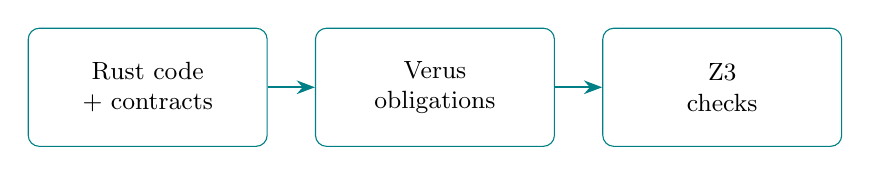
\begin{tikzpicture}[node distance=6mm,box/.style={draw=Teal,rounded corners,align=center,minimum height=15mm,text width=28mm,font=\small}]
\node[box] (s) {Rust code\\+ contracts};
\node[box,right=of s] (v) {Verus\\obligations};
\node[box,right=of v] (z) {Z3\\checks};
\draw[-{Stealth},thick,Teal] (s)--(v);
\draw[-{Stealth},thick,Teal] (v)--(z);
\end{tikzpicture}
\end{center}
\begin{itemize}
\item Write specifications and proofs alongside executable code.
\item Verify supported Rust code with annotations and library specifications.
\item Erase specification/proof code when compiling the executable.
\end{itemize}
\source{https://github.com/verus-lang/verus}{Verus project}\source{https://verus-lang.github.io/verus/guide/modes.html}{Verus Guide: code modes}
\note{Verus supports a subset of Rust; existing crates are not automatically fully verified. The diagram is conceptual, not a complete description of the internal compiler pipeline.}
\end{frame}

\begin{frame}{Three modes, three jobs}
\begin{tabular}{p{.17\textwidth}p{.38\textwidth}p{.32\textwidth}}
\toprule
Mode & Purpose & Example \\\midrule
\texttt{exec} & Actual computation & Update a counter \\\addlinespace
\texttt{spec} & Mathematical definitions & Describe the desired result \\\addlinespace
\texttt{proof} & Establish logical facts & Supply a lemma or assertion \\\bottomrule
\end{tabular}
\vspace{5mm}
\begin{itemize}
\item Think: computation, definition, and lemma.
\item Specifications can use mathematical \texttt{int} and \texttt{nat}.
\item Ghost code is reasoning-only code, erased before execution.
\end{itemize}
\source{https://verus-lang.github.io/verus/guide/modes.html}{Verus Guide: code modes}
\note{Machine integers still matter in exec code. Mathematical types let the specification describe arithmetic without silently wrapping. Proof functions can package reusable arguments.}
\end{frame}

\begin{frame}[fragile]{The counter contract in Verus}
\begin{lstlisting}
fn advance(x: u32, limit: u32) -> (r: u32)
    requires x <= limit,
    ensures
        r <= limit,
        r == (if x < limit { x + 1 } else { x }),
{
    if x < limit { x + 1 } else { x }
}
\end{lstlisting}
\begin{itemize}
\item \texttt{requires}: what callers must establish.
\item \texttt{ensures}: what callers may rely on afterward.
\item Verus also checks the executable addition for overflow.
\end{itemize}
\source{https://verus-lang.github.io/verus/guide/requires_ensures.html}{Verus Guide: contracts}
\note{The complete file adds use vstd::prelude::* and a verus! block. In specification expressions, the addition is mathematical. In the executable branch, x < limit and the u32 bound on limit justify x + 1. This is intended to be an automatically discharged example.}
\end{frame}

\begin{frame}{What must be established?}
\begin{enumerate}
\item \textbf{Safe addition:} $x<\mathit{limit}\le\texttt{u32::MAX}$ gives room to increment.
\item \textbf{Bounded result:} each branch returns at most the limit.
\item \textbf{Exact behavior:} increment below the limit, stay put at the limit.
\end{enumerate}
\begin{block}{Try the original bug}Replace \texttt{x < limit} with \texttt{x <= limit} in the body.\par The same contract should reject the implementation.\end{block}
\note{Keep the specification unchanged during this mutation. At equality the body disagrees with the exact postcondition and breaks the bound; at MAX the body can overflow as well. This is a useful demonstration even when not running live.}
\end{frame}

\begin{frame}{Using a verified function is applying a lemma}
Suppose we have established
\[
 \forall x,L\in\{0,\ldots,2^{32}-1\},\quad
 x\le L\ \Longrightarrow\ \operatorname{advance}(x,L)=\min(x+1,L).
\]
\begin{itemize}
\item Instantiate at $(x,L)=(4,5)$ to deduce the result is $5$.
\item Instantiate at $(x,L)=(5,5)$ to deduce the result is again $5$.
\item At $(x,L)=(6,5)$, the hypothesis fails; the theorem gives no guarantee.
\end{itemize}
\begin{block}{Modular proof}
Subsequent arguments use the function's contract as a lemma.\par
They need not repeat the proof about its implementation.
\end{block}
\note{The displayed functional equation is justified for this terminating function. General Hoare contracts need the partial-correctness qualification discussed earlier. The corresponding client assertions are retained in examples/counter.rs.}
\end{frame}


\begin{frame}{A loop invariant is an induction hypothesis}
For \texttt{while} $B$ \texttt{do} $C$, choose a predicate $I$ on states.
\[
 \underbrace{P\Rightarrow I}_{\text{base case}},\qquad
 \underbrace{\{I\land B\}\ C\ \{I\}}_{\text{inductive step}},\qquad
 \underbrace{I\land\neg B\Rightarrow Q}_{\text{conclusion at exit}}.
\]
For repeated bounded successor, take $I(x)\equiv 0\le x\le L$.
\begin{itemize}
\item Initially: $0\le x_0\le L$ is assumed.
\item If $x<L$, then $x'=x+1\le L$; the invariant is preserved.
\item At exit: $x\le L$ and $\neg(x<L)$ imply $x=L$.
\end{itemize}
\begin{block}{Termination uses well-foundedness}
$V(x)=L-x\in\mathbb{N}$ decreases strictly on every iteration.
\end{block}
\note{Induct on the number of completed iterations. The invariant includes the state where the guard is false, so x < L would be too strong. Nonnegativity is implicit for u32 in the upcoming code. A strictly descending sequence in the naturals cannot be infinite; this is the separate termination argument.}
\end{frame}

\begin{frame}[fragile]{Loops need an invariant}
\begin{lstlisting}[basicstyle=\ttfamily\footnotesize]
fn fill_to_limit(start: u32, limit: u32) -> (r: u32)
    requires start <= limit,
    ensures r == limit,
{
    let mut x = start;
    while x < limit
        invariant x <= limit,
        decreases limit - x,
    {
        x = advance(x, limit);
    }
    x
}
\end{lstlisting}
\small Invariant: we stay within the limit. Variant: the remaining distance shrinks.
\source{https://verus-lang.github.io/verus/guide/while.html}{Verus Guide: Loops and invariants}
\note{Deliberately simple, not a recommended implementation of assignment. Establish the invariant initially, preserve it after each step, then combine it with the negated guard to get equality. The variant is nonnegative and strictly decreases while the guard holds.}
\end{frame}

\begin{frame}{What is being trusted?}
\begin{itemize}
\item The specification captures the intended theorem.
\item The translation from code to logical obligations is sound.
\item The solver's result and any assumed lemmas are correct.
\item Compilation and execution preserve the verified meaning.
\end{itemize}
\begin{block}{Distinguish proof search from proof checking}
Here we rely on the Verus/Z3 verification pipeline.\par
We are not presenting an independently checked proof certificate.
\end{block}
\note{This is a natural question for an audience familiar with proof assistants. Explain the trust boundary of this workflow without implying that SMT solvers cannot produce proofs or that other proof systems have no trusted components. Our demonstration runs verification; it does not export a certificate to a separate small kernel.}
\end{frame}

\section{Verification as LLM Guardrails}
\begin{frame}{An LLM proposes a construction; verification checks it}
\begin{center}
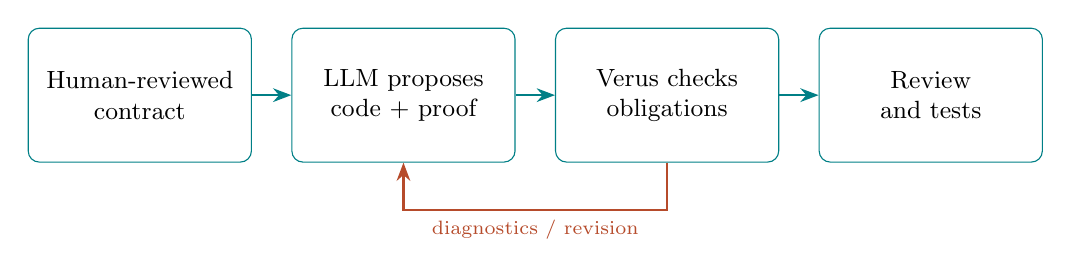
\begin{tikzpicture}[node distance=5mm,box/.style={draw=Teal,rounded corners,align=center,minimum height=17mm,text width=26mm,font=\small}]
\node[box] (s) {Human-reviewed\\contract};
\node[box,right=of s] (l) {LLM proposes\\code + proof};
\node[box,right=of l] (v) {Verus checks\\obligations};
\node[box,right=of v] (r) {Review\\and tests};
\draw[-{Stealth},thick,Teal] (s)--(l);
\draw[-{Stealth},thick,Teal] (l)--(v);
\draw[-{Stealth},thick,Teal] (v)--(r);
\draw[-{Stealth},thick,Rust] (v.south) -- ++(0,-.6) -| node[pos=.25,below,font=\scriptsize]{diagnostics / revision} (l.south);
\end{tikzpicture}
\end{center}
\vspace{6mm}
\large Plausibility is not a proof: check the generated construction against a fixed claim.
\note{This is a proposed engineering workflow, not a claim that Verus guarantees all LLM output is safe. LLMs can help draft implementations, invariants, and lemmas; the generated proof text itself is not evidence until checked.}
\end{frame}

\begin{frame}{A concrete revision loop}
\begin{enumerate}
\item Freeze the counter contract and allowed input domain.
\item Ask the LLM to implement the function and discharge obligations.
\item Reject the \texttt{<=} candidate when verification fails.
\item Revise the body to use \texttt{<}; check the same contract again.
\item Inspect the changed argument and test the surrounding program.
\end{enumerate}
\begin{block}{Helpful prompt constraint}``Keep the contract unchanged. Do not introduce assumptions or bypass verification. Explain any remaining obligations.''\end{block}
\note{A prompt constraint helps communicate intent but is not enforcement. Repository permissions, review, and CI must enforce the acceptance policy independently. Do not let an agent edit the verifier command to make a failed run appear successful.}
\end{frame}

\begin{frame}{Do not let a proof attempt change the theorem}
\begin{itemize}
\item \textbf{Weaken the conclusion:} replace $r=\min(x+1,L)$ by $r\le L$.
\item \textbf{Strengthen the hypotheses:} exclude the failing boundary case.
\item \textbf{Assume the claim:} introduce an unproved premise that implies it.
\end{itemize}
\begin{block}{The guardrail must preserve the statement}
Fix the contract, audit new assumptions, and require all intended obligations to pass.
\end{block}
\note{These are familiar mathematical ways to prove something other than the original claim. An LLM repair loop can make the same moves. Review hypothesis changes even when they remain consistent. Tool errors and timeouts must not be counted as successful verification. Preserve the command, tool versions, and exact submitted code.}
\end{frame}

\begin{frame}{The guardrail has a defined reach}
\begin{columns}[T]
\column{.48\textwidth}
\begin{block}{Can establish, when specified}
\begin{itemize}
\item Results satisfy a contract.
\item Arithmetic stays in range.
\item A modeled invariant is preserved.
\end{itemize}
\end{block}
\column{.48\textwidth}
\begin{block}{Still needs separate evidence}
\begin{itemize}
\item The contract matches user intent.
\item External systems match the model.
\item The algorithm is efficient enough to use.
\end{itemize}
\end{block}
\end{columns}
\vspace{6mm}
\large Stronger acceptance criteria make generated code easier to evaluate.
\note{Verification is especially valuable when humans can describe the invariant more reliably than they can inspect every generated implementation. Properties omitted from the contract remain outside the claim.}
\end{frame}

\begin{frame}{Start with one property worth keeping true}
\begin{enumerate}
\item Write the contract before polishing the implementation.
\item Use Z3's counterexample-search model to understand proof obligations.
\item Let Verus connect those obligations to Rust code.
\item Make verification a required check for LLM-generated changes.
\end{enumerate}
\vspace{6mm}
\Large Which theorem about an algorithm would you want its implementation to carry?
\note{Invite questions. Possible mathematical examples: a sorting routine preserves the input multiset, Euclid steps preserve the gcd, or a numerical method maintains a certified error bound. Each requires a specification and an appropriate model of arithmetic; floating-point analysis requires additional care.}
\end{frame}

\begin{frame}{References and demo files}
\small
\begin{itemize}
\item \href{https://verus-lang.github.io/verus/guide/}{Verus Tutorial and Reference}\par\scriptsize\url{https://verus-lang.github.io/verus/guide/}\small
\item \href{https://github.com/verus-lang/verus}{Verus source and installation instructions}\par\scriptsize\url{https://github.com/verus-lang/verus}\small
\item \href{https://microsoft.github.io/z3guide/}{Microsoft's Z3 Guide}\par\scriptsize\url{https://microsoft.github.io/z3guide/}\small
\end{itemize}
\medskip
Local examples: \texttt{examples/counter.rs},\par
\texttt{examples/counter-bug.smt2}, \texttt{examples/counter-fixed.smt2}.
\note{The README documents build commands and validation status. Source links throughout the deck are clickable. Speaker notes live in the TeX source and are hidden in the audience PDF.}
\end{frame}
\end{document}
